\documentclass[tikz]{standalone}
\usepackage{amsmath}
\usepackage{pgf}
\usepackage{pgfplots}
\pgfplotsset{compat=1.18,}
\usepgfplotslibrary{fillbetween}
% \listfiles
\begin{document}
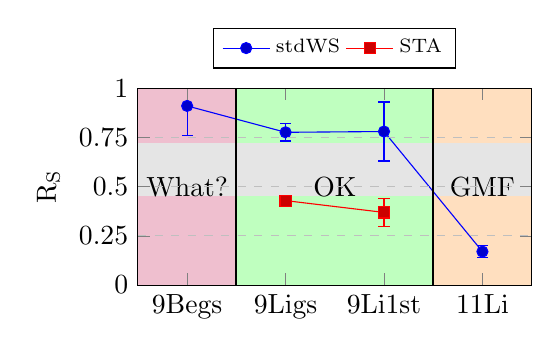
\begin{tikzpicture}[
		% trim left=-20,
	]
	\begin{axis}[
		width=5cm,
		height=2.5cm,
		scale only axis,
		ylabel={$\text{R}_{\text{S}}$},
		% minor y tick num=1,
		xticklabels={9Begs, 9Ligs, 9Li1st, 11Li},
		xtick={0,1,2,3},
		xmin=-0.5, xmax=3.5,
		ymin=0, ymax=1,
		ymajorgrids=true, yminorgrids=false,
		ytick distance=0.25,
		legend style={
				fill=none,
				anchor=south,
				at={(0.5, 1.1)},
				font=\scriptsize,
			},
		legend columns=3,
		grid style={dashed},
		axis on top,
		% fill between/on layer={main},
		]
		\addplot[fill=black!10, draw=none, forget plot] coordinates {(\pgfkeysvalueof{/pgfplots/xmin}, 0.45) (\pgfkeysvalueof{/pgfplots/xmax}, 0.45)  (\pgfkeysvalueof{/pgfplots/xmax}, 0.72) (\pgfkeysvalueof{/pgfplots/xmin}, 0.72)};
		\addplot+ [
			error bars/.cd,
			y dir=both,y explicit,
		] coordinates {
				(0, 0.91) +- (0, 0.15)
				(1, 0.776) +- (0, 0.044)
				(2, 0.78) +- (0, 0.15)
				(3, 0.170) +- (0, 0. 031)
			};
		\addplot+ [
			error bars/.cd,
			y dir=both,y explicit,
		] coordinates {
				(1, 0.429) +- (0, 0.024)
				(2, 0.369) +- (0, 0.072)
			};
		%% Left of axis
		\path[name path=laxis] (\pgfkeysvalueof{/pgfplots/xmin}, 0) -- ( \pgfkeysvalueof{/pgfplots/xmin}, \pgfkeysvalueof{/pgfplots/ymax});
		%% Right of axis
		\path[name path=raxis] (\pgfkeysvalueof{/pgfplots/xmax}, 0) -- ( \pgfkeysvalueof{/pgfplots/xmax}, \pgfkeysvalueof{/pgfplots/ymax});
		%% Left separation
		\addplot[black, thick, name path=right] coordinates {(2.5, \pgfkeysvalueof{/pgfplots/ymin} ) (2.5, \pgfkeysvalueof{/pgfplots/ymax})};
		%% Right separation
		\addplot[black, thick, name path=left] coordinates {(0.5, \pgfkeysvalueof{/pgfplots/ymin} ) (0.5, \pgfkeysvalueof{/pgfplots/ymax})};
		%% Fillings
		% 1 Left
		\addplot[purple!25] fill between [of=laxis and left];
		% 2 Middle
		\addplot[green!25] fill between [of=left and right];
		% 3 Right
		\addplot[orange!25] fill between [of=right and raxis];
		% Annotations
		\node at (axis cs:0,0.5) {What?};
		\node at (axis cs:1.5,0.5) {OK};
		\node at (axis cs:3,0.5) {GMF};
		\legend{stdWS, STA}
	\end{axis}
\end{tikzpicture}
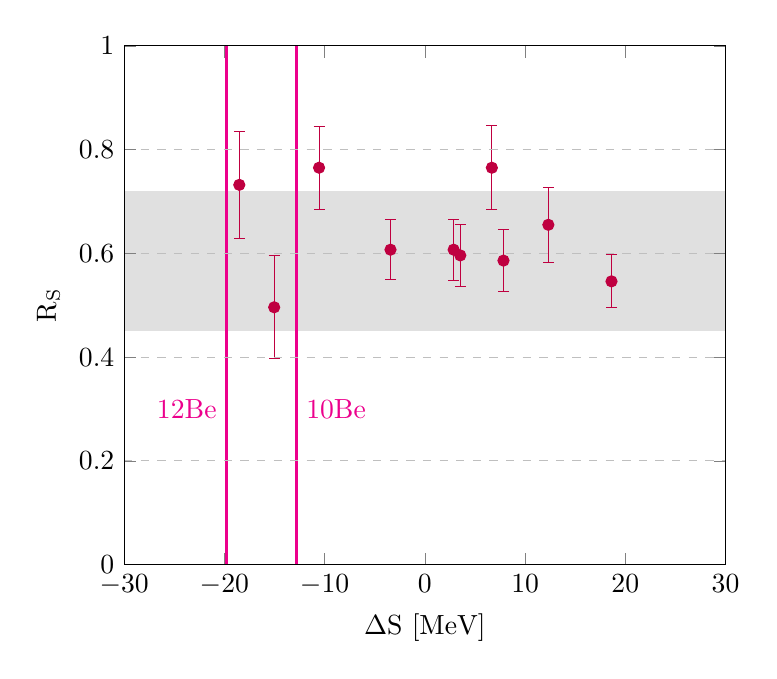
\begin{tikzpicture}
	\begin{axis}[
		width=0.63\linewidth,
		scale only axis,
		xlabel={$\Delta$S [MeV]},
		ylabel={$\text{R}_{\text{S}}$},
		xmin=-30, xmax=30,
		ymin=0, ymax=1,
		ymajorgrids=true, yminorgrids=true,
		grid style = {dashed},
		axis on top,
		]
		\addplot[fill=black!12, draw=none, forget plot] coordinates {(\pgfkeysvalueof{/pgfplots/xmin}, 0.45) (\pgfkeysvalueof{/pgfplots/xmax}, 0.45)  (\pgfkeysvalueof{/pgfplots/xmax}, 0.72) (\pgfkeysvalueof{/pgfplots/xmin}, 0.72)};
		\addplot [purple, only marks,
			error bars/.cd,
			y dir=both, y explicit,
		] table [y error=u] {
				x		   y      u
				-18.508    0.732  0.103
				-15.028    0.496  0.099
				-10.552    0.765  0.080
				-3.425    0.607  0.058
				2.873    0.607  0.059
				3.536    0.596  0.060
				6.685    0.765  0.081
				7.845    0.586  0.060
				12.320    0.655  0.072
				18.619    0.546  0.051
			};
		\draw[magenta, very thick] (axis cs:-12.8,\pgfkeysvalueof{/pgfplots/ymin}) -- (axis cs:-12.8,\pgfkeysvalueof{/pgfplots/ymax});
		\node[magenta, right] at (-12.8, 0.3) {10Be};
		\draw[magenta, very thick] (axis cs:-19.8,\pgfkeysvalueof{/pgfplots/ymin}) -- (axis cs:-19.8,\pgfkeysvalueof{/pgfplots/ymax});
		\node[magenta, left] at (-19.8, 0.3) {12Be};
	\end{axis}
\end{tikzpicture}
\end{document}